\documentclass[letterpaper,12pt]{article}
 
\usepackage[spanish]{babel}
\usepackage[utf8]{inputenc}
\usepackage{pdfpages}
\usepackage{rotating}
\usepackage{color}
\usepackage{amsmath}
\usepackage{multicol}
\usepackage{graphicx}     % permite insertar figuras
\usepackage{fancyhdr}   % para encabezado y pie de pagina
\usepackage{listings}   % para escribir codigo
\usepackage{hyperref}   % crea links en el indice y notas al pie.
\usepackage{float}         % permite dejar las imagenes es una posición fija    
\usepackage{anysize}     % Permite emplear cualquier medida de márgenes.
   \marginsize{2cm}{2cm}{1cm}{1cm} 
% Controla los márgenes {izquierda}{derecha}{arriba}{abajo}. 


    %\pagestyle{fancy}
 
 
\begin{document}
 
 \begin{titlepage}
	\begin{figure}[h!]
		
\includegraphics[width=0.4\textwidth]{fcfm}
		\vspace{0.75cm} 
	\end{figure}
        \hspace*{2.3cm} 

        \bigskip

        \vspace*{4 cm}
        \begin{center}
            \huge{Informe Final: HappyDent}\\
	\large{EL6020 – Taller de Innovación Tecnológica y Emprendimiento}
        \end{center}
        \vspace*{3 in}
        \begin{flushright}
            \begin{tabular}{ll}
		
                \textbf{\textit{Alumnos}} &: Felipe Barrera\\
					&: Angelo Falchetti\\
					&: Roberto Fuentes\\
		\textbf{\textit{Profesor}} &: Alberto Compagnon \\
		\textbf{\textit{Profesor Auxiliar}} &: Mario Medina \\
                \textbf{\textit{Fecha}} &: \today \\
            \end{tabular}
        \end{flushright}
    \end{titlepage}

\newpage
 
\section{Resumen}

La odontofobia es una de las causas de la no asistencia de las personas a realizarse controles dentales preventivos. 
Es por ello que la empresa HappyDent busca combatir la odontofobia mediante la aislación del ruido emitido por las microturbinas y los micromotores utilizados en las consultas odontológicas, ruido que provoca estrés y ansiedad tanto en el usuario que está siendo atendido como en el que espera la atención. 
\\[0.5cm]
\indent Además se observa que otro de los factores de la no asistencia es la falta de tiempo y motivación a la hora de solicitar horas de atención.
Se estima que la mejora en la atención, ya sea por el control del ruido como la comodidad de la aplicación, aumentará en un 23\% la cantidad de usuarios que se realizarían controles dentales preventivos, lo que genera un aumento en los ingresos de las consultas que sean adaptadas por la empresa debido al aumento de la demanda. 
Además se espera que la demanda siga aumentando debido a los buenos comentarios que se tengan en relación a la calidad de servicio que entrega la consulta odontológica.
\\[0.5cm]
\indent El VAN de la empresa por concepto de implementación de los audífonos de aislación es de \$487 millones de pesos chilenos, a una tasa de descuento del 15\%.
\\[0.5cm]
\indent Actualmente en Chile no existe un producto similar. 
Lo cual convertirá a la empresa HappyDent en los pioneros en mejorar la calidad de la atención de las consultas en el ámbito del ruido generado por el instrumental de éstas. 
Además será el pionero en desarrollar una aplicación para Smartphone para reserva de horas de atención.
\\[0.5cm]
\indent El beneficiario último es el usuario de las consultas, quien tendrá una placentera visita al dentista. 
Incluso quienes no presentan fobias en la visita al odontólogo saldrán beneficiados, ya que no escucharan el sonido del instrumental.
\\[0.5cm]
\indent El dispositivo será vendido a las universidad, centros dentales, hospitales, consultorios y clinicas privadas. 
Quien adquiera el servicio, podrá diferenciarse de sus competidores y proveer de un servicio de mayor calidad. 
El acceso a la aplicación se dividirá en dos segmentos: las consultas y los usuarios quienes las descarguen, siendo pagada para el primero y gratis para el segundo.
\\[0.5cm]
\indent El mercado al cual se apunta es de alrededor de 18.000 dentistas ya profesionalizados y anualmente egresan 1.200 nuevos profesionales. 
Un aumento de tal magnitud entrega dos grandes beneficios:

	\begin{itemize}
		\setlength{\itemsep}{0pt}%
		\setlength{\parskip}{0pt}%
		\item El aumento de los clientes.
		\item Nuevos profesionales jóvenes quienes tienen más afinidad con los avances tecnológicos.
	\end{itemize}

\indent El producto contará con distintos niveles de servicio, para poder satisfacer las necesidades de todos los clientes. 
Desde el simple dispositivo para atenuar el sonido, hasta disfrutar de un conjunto de distracciones que permitan hacer olvidar dónde se encuentra el paciente.

%%%%%%%%%%%%%%%% 
	\newpage
	\tableofcontents
	\newpage
%%%%%%%%%%%%%%%%

\section{Emprendimiento}
Una de los problemas observados en las consultas dentales es la odontofobia que presentan 
algunos pacientes, que consiste en un miedo a la misma consulta dental y los tratamientos que en 
ellas se hace. Este miedo puede abarcar uno o más de los elementos presentes en las consultas: el 
usuario puede tener miedo hacia el dentista, la instrumentación utilizada, la silla de procedimientos, 
la falta de control durante el procedimiento o los ruidos generados por los instrumentos utilizados.
\\[0.5cm]
\indent Dado lo anterior surge la idea de convertir la visita al dentista en una experiencia grata, de manera de evitar total o gradualmente la odontofobia que presentan algunos de los usuarios de las 
consultas dentales. Esto implicará una mejora tanto en la psiquis de los pacientes, que podrán 
relajarse durante las consultas, como en su salud dental, ya que disminuir su aversión a esta 
experiencia incrementará su asistencia a la consulta. De forma paralela, la salud de los doctores y 
otros trabajadores de la consulta también puede cuidarse mediante la introducción de medidas 
análogas para ellos, que este proyecto también abarca.
\\[0.5cm]
\indent Uno de los factores que se quiere mejorar con el proyecto es la aislación del ruido emitido por las microturbinas y los micromotores que se utilizan en los tratamientos, principalmente de limpieza de las piezas dentales. Este será el foco inicial del emprendimiento, sin perjuicio de que en un futuro la línea de trabajo pueda expandirse acorde a la misión establecida por la organización.
\\[0.5cm]
\indent Para lograr lo expuesto anteriormente, se diseñarán tres formas distintas de la aislación del ruido, que van asociadas directamente en el nivel de especificidad de dicha aislación: si aislar el ruido desde la microturbina; que el paciente no escuche el ruido mediante audífonos o una aislación acústica de la sala de atención.
\\[0.5cm]
\indent Las principales funcionalidades del proyecto se detallan a continuación:

	\begin{itemize}
		\setlength{\itemsep}{0pt}%
		\setlength{\parskip}{0pt}%
		\item Silenciador: complemento a la microturbina y micromotor que aísla localmente el ruido emitido por estos instrumentos.
		\item Audífonos: destrucción de la frecuencia del ruido que emiten la microturbina y el micromotor. Al ser una destrucción específica de frecuencias, permite escuchar las otras frecuencias, como lo es la emitida por la voz humana.
		\item Aislación sala de atención: evitar la emisión del ruido provocado dentro de la sala de atención hacia las otras dependencias de la consulta. Esto evita que los usuarios que están esperando la atención sientan ansiedad por el molesto ruido de los instrumentos.
		\item Aplicación para Smartphone que permita la reserva y consulta de horas por parte de los clientes de las consultas odontológicas. Esto permitirá a la consulta tener publicidad dentro de la aplicación y una nueva plataforma para la solicitud de horas.
	\end{itemize}

\indent El objetivo del proyecto, como ya se ha implicado antes, es mejorar la calidad de atención de
la consulta odontológica. Por ende, el público objetivo serán las consultas que deseen mejorar la 
atención que les brinda a sus clientes. Además de mejorar la atención a los clientes, se mejorará el 
ambiente laboral de sus trabajadores, ya que los productos ofrecidos podrán ser utilizados por los 
integrantes de la consulta, que involucran al dentista, auxiliares de los dentistas, secretarias 
recepcionistas y auxiliares de aseo. Con la implantación de la aplicación aumentará los canales para 
la solicitud de horas, lo que aumentará la cantidad de clientes que tengan las consultas que 
contraten el servicio.
\\[0.5cm]
\indent Este proyecto aporta varios valores agregados al mercado de las consultas dentales
existente, tanto para los trabajadores como para los pacientes, pudiéndose identificar con mayor 
claridad los siguientes:
	\begin{itemize}
		\setlength{\itemsep}{0pt}%
		\setlength{\parskip}{0pt}%
		\item Re-experimentar la consulta dental de manera positiva.
		\item Mejorar la salud dental del país.
		\item Mejorar la salud auditiva de los trabajadores de las consultas dentales.
		\item Mejorar el proceso de solicitud de horas.
	\end{itemize}

\indent En general la aplicación dispondrá de la siguiente operación:

	\begin{figure}[h!]
		\begin{center}
			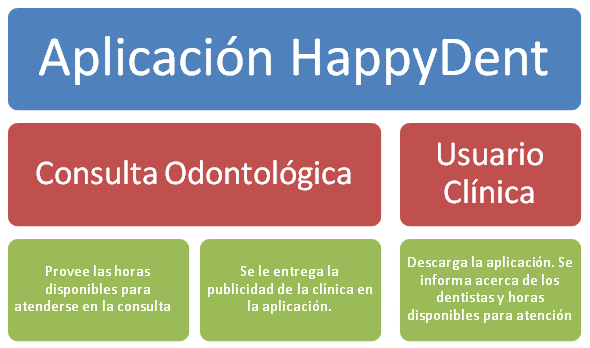
\includegraphics[width=0.8\textwidth]{op_aplicacion_cel}
			\caption{Operación de la aplicación para Smartphone.}
			\label{smatphone}
		\end{center}
	\end{figure}
	\newpage
	\subsection{Misión, visión y objetivos estratégicos}

Siempre es importante tener un horizonte claro sobre qué busca la organización del proyecto,
lo que queda plasmado en la misión y visión del emprendimiento. Además, se plantean objetivos 
estratégicos sobre la implementación de la idea en un plazo real.
		\subsubsection{Misión}
		
			\begin{center}
				{\color{blue} ``Usar los avances tecnológicos para mejorar la salud dental y auditiva del país,mediante la transformación de la experiencia en la consulta dental tanto para los pacientes como para lostrabajadores".}
			\end{center}

		\subsubsection{Visión}
				\begin{center}
				{\color{blue} ``Ser los mayores proveedores de tecnología para el alivio emocional en las consultas dentales del país, admirados por nuestra confiabilidad y calidad de servicio".}
			\end{center}

		\subsubsection{Objetivos Estratégicos}

Los objetivos estratégicos de la empresa buscan entrar en el mercado de manera eficaz y
consolidarse como líder en mejorar la calidad de la experiencia en las consultas dentales. Para ello 
se buscará

			\begin{itemize}
				\setlength{\itemsep}{0pt}%
				\setlength{\parskip}{0pt}%
				\item Adaptar 3000 consultas dentales en los próximos 5 años.
				\item Lograr 20.000 descargas dentro de los próximos 5 años.
				\item Construir una reputación sólida como proveedor confiable y capaz de resolver problemas.
				\item Diseñar nuevos sistemas para reducir la tensión en las personas en las consultas dentales.
			\end{itemize}
	\newpage
	\subsection{Plan de Negocios}

El plan de negocios del proyecto se puede resumir en el siguiente canvas:

		\begin{figure}[h!]
			\begin{center}
				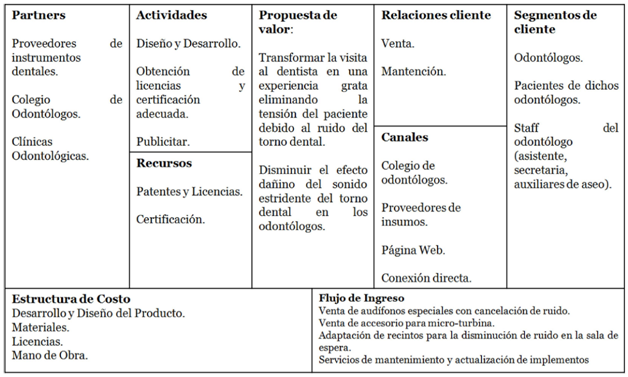
\includegraphics[width=0.75\textwidth]{canvas}
				\caption{Canvas del plan de negocio de la empresa.}
				\label{canvas}
			\end{center}
		\end{figure}

	\subsection{Análisis de proyecto}

Ya establecida la idea general del proyecto es importante resolver aquellas partes que
requieren mayor atención, para conocer las fortalezas y debilidades que se tiene. Para ello se 
realizan dos tipos de análisis: un análisis de Porter que enfatiza el estado del mercado y los distintos agentes que actúan en él, y un análisis DAFO/CAME, fortalecer la implementación del proyecto.
		\newpage
		\subsubsection{Fuerzas de Porter}
			\begin{figure}[h!]
				\begin{center}
					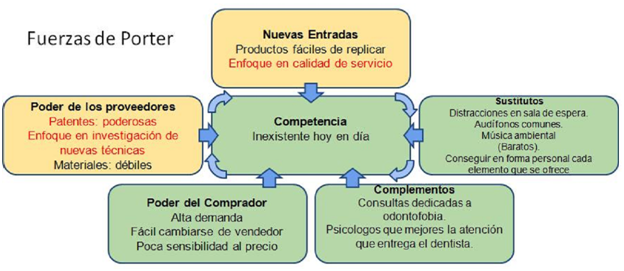
\includegraphics[width=0.8\textwidth]{porter}
					\caption{Fuerzas de Porter.}
					\label{porter}
				\end{center}
			\end{figure}

En la figura \ref{porter} se muestran las distintas fuerzas que los agentes aplican sobre el
mercado del proyecto. En ella se indica que todos los factores son relativamente positivos (lo que 
indica un buen negocio), pero además se indican algunos detalles a cuidar.
\\[0.5cm]
\indent Por un lado se observa que nuevos competidores pueden entrar fácilmente al mercado 
copiando los productos, que no son difíciles de replicar. Para combatir esta fuerza se le dará un 
enfoque de servicio al proyecto, donde la lealtad de los clientes juegue un factor importante. Esto 
añade un rol difícil de replicar por otros competidores, que mantendrá al proyecto a la delantera. 
Además se recordará siempre el patentar todas las ideas nuevas que se generen dentro del 
emprendimiento, de manera de regular a la competencia mediante el cobro de licencias.
\\[0.5cm]
\indent Por otro lado, se observa que los proveedores de propiedad intelectual pueden ser 
poderosos, ya que existen pocos competidores en estas tecnologías. Es por esto que es importante 
desarrollar un equipo de investigación por lo menos en el mediano plazo, de manera de 
independizarnos lo antes posible de las patentes externas, para pasar a ser los proveedores de las 
mejores técnicas.
\\[0.5cm]
\indent En las otras áreas se observan detalles menos cruciales, como la facilidad de cambiarse de 
vendedor por parte de los compradores, pero esto se combate de igual manera con el programa de 
lealtad antes mencionado. Los clientes directos (odontólogos) tienen un capital de inversión para 
instrumentos elevado en comparación al precio que los distintos productos vendidos, por lo que 
diferencias en el precio de los productos toman un rol menor en comparación de la calidad de 
servicio. De la misma manera, la opción sustituta de comprar cada elemento por separado y 
preocuparse por sí mismo de las instalaciones en general no se justifica.
		\newpage
		\subsubsection{Análisis DAFO y CAME}
Con el siguiente análisis se generan listas de acciones a seguir para fortalecer el negocio.
\newpage
\section{Mercado}

El mercado al cual se apunta es el mundo odontológico en Chile. Ya sean clínicas
particulares, hospitales, centros asistenciales o universidades. O sea, donde un dentista atiende 
pacientes. El otro mercado al que se apunta es el relativo a las descargas de aplicaciones para 
Smartphone.
\\[0.5cm]
\indent Actualmente se estima que hay más de 18.000 dentistas practicando su oficio y cada año 
egresan aproximadamente 1.200 nuevos profesionales. Los dentistas se distribuyen entre el área de 
atención privada y pública. De acuerdo con las estadísticas encontradas\footnote{Dr. Sergio Coisiño M., Consejero Nacional, Colegio de Cirujano Dentistas de Chile. ``¿Cuántos somos
actualmente los dentistas en Chile?", CONTRAANGULO, revista capítulo de odontólogos de libre ejercicio. 2 de julio de 2013.}, el 85\% de la población se
atiende en el área pública, mientras que el 15\% restante lo hace de forma privada. Actualmente 
trabajan cerca de 4.200 dentistas en el sector público atendiendo a casi catorce millones de 
pacientes. Dejando a cerca de 12.000 dentistas del sector privado apuntando a un poco más de dos 
millones de potenciales pacientes.
\\[0.5cm]
\indent El mercado relativo a las aplicaciones para teléfonos inteligentes es creciente y muy fuerte en las generaciones jóvenes, por lo cual la implantación del servicio dentro de la comunidad de usuarios de consultas odontológicas será factible.
\\[0.5cm]
\indent El proyecto apunta a mejorar la experiencia que el paciente experimenta en la consulta, 
considerando en primera instancia a disminuir los ruidos molestos que se pueden experimentar 
durante la consulta. En segunda instancia se busca mejorar la comodidad del usuario de las consultas al momento de solicitar horas. Se mantiene la tónica de que no existen competidores que
hayan implementado una aplicación para la solicitud de horas en consultas odontológicas.
\\[0.5cm]
\indent Se tendrá al mercado sólo para la empresa por un breve periodo de tiempo, ya que no hay 
otro agente que cubra la necesidad. Durante este periodo se tendrá un feedback de parte de los 
clientes, lo cual permitirá mejorar la versión. Para obtener esta información, cualquier proyecto 
competidor deberá emplear tiempo, que tiene un costo y un retraso que se debe aprovechar. La 
ausencia de competidores baja la barrera de entrada permitiendo el ingreso de nuevos actores al 
mercado.
\\[0.5cm]
\indent A partir de una encuesta realizada dentro de los estudiantes de la universidad, se observó 
que un tercio admite sentir estrés en su experiencia dental, de entre los cuales la mitad anotó 
sentirse molesto por el ruido de los instrumentos. Sin perjuicio de este resultado, más del 50\% 
responde que les sería más placentera la experiencia si el ruido fuese eliminado. Esto indica que el 
proyecto efectivamente tiene el potencial de hacer un impacto en el mercado, tanto en su incursión 
inicial, como en posibles expansiones que tomen en consideración otros factores. Además, un 23\% 
declara que aumentaría su frecuencia si no escuchara el ruido, lo que no deja de ser un porcentaje 
interesante para los dentistas que pagarán el servicio.
\\[0.5cm]
\indent En base a lo ya expuesto, se observa que los dentistas del sector privado parecen ser los 
clientes más prometedores, ya que en su mercado existe una mayor competencia de dentistas y una 
menor porción de pacientes, que además acceden a este sistema buscando una mejor atención, por 
lo que el servicio ofrecido representa una alternativa atractiva como mecanismo de diferenciación. Se observa, sin embargo, que acorde con la misión del proyecto, no se busca descartar al resto del 
mercado, ya que idealmente todo el mundo podrá vivir una mejor experiencia.
\\[0.5cm]
\indent En base a lo ya expuesto, se observa que los dentistas del sector privado parecen ser los
clientes más prometedores, ya que en su mercado existe una mayor competencia de dentistas y una 
menor porción de pacientes, que además acceden a este sistema buscando una mejor atención, por 
lo que el servicio ofrecido representa una alternativa atractiva como mecanismo de diferenciación. Se observa, sin embargo, que acorde con la misión del proyecto, no se busca descartar al resto del 
mercado, ya que idealmente todo el mundo podrá vivir una mejor experiencia.
\\[0.5cm]
\indent Se establece una segmentación tentativa del mercado que abarca tres áreas:

	\begin{enumerate}
		\setlength{\itemsep}{0pt}%
		\setlength{\parskip}{0pt}%
		\item Operación pública: la cual buscará que ante un mínimo costo se mejore en alguna medida la calidad de sus atenciones.
		\item Estándar: buscará que su atención mejore de manera importante, lo cual le permite obtener un crecimiento en la demanda.
		\item Premium: buscará diferenciarse en gran medida del resto, mediante la utilización de técnicas más sofisticadas como lo es la experiencia con Oculus Rift, suscripciones a videos y música relajante, silla masajeadora, etc., de manera que la experiencia pase a ser un placer más que una consulta dental.
	\end{enumerate}

\newpage
\section{Plan de Marketing}

El producto entregado por la empresa es la mejora en la calidad de la experiencia en las
consultas dentales, mediante la entrega de implementos que abarcan audífonos anti-ruido, aislador 
de la emisión del ruido de la microturbina y aislación de la sala de procedimientos. Además se busca 
la mejora en la toma de horas y publicidad de las consultas dentales.
\\[0.5cm]
\indent La publicidad y promoción del servicio se entenderá como una estrategia de “puerta a 
puerta”, ya que se presentará personalmente a las consultas odontológicas. Igualmente se tendrá 
una plataforma web que permitirá a los clientes ya asociados poder contactarse de manera más 
rápida con la empresa que brinda el servicio. Además en esta plataforma web podrá encontrar los 
nuevos servicios que pueden ser implementados en las consultas. 
\\[0.5cm]
\indent Respecto a la aplicación, la promoción será a través de las mismas consultas odontológicas, 
las cuales podrán ofrecer el servicio de descarga de la aplicación. Otra forma de publicidad será en 
los medios escritos (revistas y diarios).
\\[0.5cm]
\indent Finalmente, se buscará un espacio de publicidad al nombre de la empresa dentro de las 
páginas web de las consultas que la posean y a través de la misma descarga de la aplicación.

	\subsection{Encuestas}

Dentro del plan de marketing, uno de los puntos fuertes es realizar encuestas a los clientes
directos y a los potenciales clientes indirectos. El plan consistió en realizar en una primera instancia una encuesta a los potenciales clientes indirectos, que en este caso corresponden a los usuarios de las consultas dentales. Con los resultados de esta encuesta se realizó una segunda encuesta enfocada a los clientes directos del proyecto, que son los dueños de consultas dentales.
		\subsubsection{Encuesta a usuarios de consultas dentales}

La encuesta buscó analizar la apreciación de los usuarios respecto a las consultas dentales y 
además analizar la importancia del valor agregado que dará el proyecto a las consultas dentales. 
\\[0.5cm]
\indent Los resultados de la encuesta se muestran en los anexos, sección 10.2.1. 
\\[0.5cm]
\indent A partir de los comentarios realizados por los encuestados en el proceso, se destacan tres 
que se repitieron y captan la atención:

			\begin{itemize}
				\setlength{\itemsep}{0pt}%
				\setlength{\parskip}{0pt}%
				\item Una de las razones por la que los pacientes no van a la consulta es por la falta de tiempo y motivación de tomar la hora e ir al dentista. Este inconveniente se podría reducir mediante una aplicación para celulares que indique cuando corresponde ir a hacerse un chequeo recomendado, dónde conviene hacerlo (indicando los precios de varios centros y su disponibilidad de productos HappyDent), además de la posibilidad de coordinar y reservar una hora de manera automática mediante el cruce de horas disponibles y la agenda personal del usuario. Se observa que esta aplicación no tiene que referirse sólo a la salud dental, sino que también puede aplicarse a la consulta oftalmológica u otras. Incluso, pensando de manera extrema, podría generarse un sistema de traslado adecuado (e.g. taxis) de forma automática.
				\item Otra fuente de molestias recurrente es la falta de control durante los procedimientos, por lo que vale la pena investigar opciones de comunicación paciente-doctor que alivien dicha sensación. En particular, una idea es entregarle al paciente un botón que éste pueda apretar en caso de sentir demasiado dolor, de manera de comunicarle al doctor sobre su situación (para que así éste tome medidas adecuadas).
				\item Una tercera molestia mencionada por los encuestados es la sensación de desinformación o poca claridad de los detalles del procedimiento. Para esto, son los dentistas quienes deben ser más claros y lograr entender si sus pacientes están conformes con sus explicaciones; para ello, los complementos del negocio entran en efecto, tanto a nivel de educación universitaria, como de coaching de psicólogos. Como idea de negocio, en este caso se puede hacer una relación adicional con los dentistas de manera de complementar sus explicaciones con vídeos/gráficos/modelos ilustrativos (e instalar monitores y programas computacionales adecuados). Para ello, se pueden aceptar peticiones por parte del personal sobre material audiovisual que les sea útil, teniendo un equipo de expertos en presentaciones que logren capturar las ideas de los doctores, quienes no tienen tiempo (o a veces habilidades) suficientes para hacer este material. En esta misma línea, usando información de los rayos X tomados de los mismos pacientes, se podrían generar modelos 3D que indiquen el procedimiento específico que se le realizará al paciente en particular (con gráficos explícitos usando un modelo de su propia boca).
			\end{itemize}


Tras los comentarios obtenidos, la empresa optó por la implementación en el corto plazo de
una aplicación para Smartphone, la cual es detallada a lo largo del informe. 
\\[0.5cm]
\indent Naturalmente, los otros avances no necesariamente se harán de forma inmediata, sino que 
son propuestas de expansión a contemplar por la organización.

		\subsubsection{Encuesta a dueños de consultas dentales}

Posterior a la encuesta realizada a los clientes indirectos del servicio, que son los usuarios de
las consultas odontológicas, se realizó un análisis de la apreciación del servicio por parte de los 
clientes directos que se tendrán. La encuesta siguió la siguiente estructura:
		\begin{enumerate}
			\setlength{\itemsep}{0pt}%
			\setlength{\parskip}{0pt}%
			\item Rubro al que pertenece: clínica privada, hospital público, consulta particular, escuela odontológica.
			\item Apreciación de los clientes ante el servicio entregado: cantidad y contenido de los reclamos y/o sugerencias recibidas.
			\item Presentación del servicio a entregar.
			\item Indexación de la demanda adicional que tendrían por concepto de mejorar el servicio.
			\item Análisis de la aceptabilidad por parte de la consulta al servicio a contratar. Los resultados específicos de la encuesta se adjuntan en el anexo 10.2.2.2.
		\end{enumerate}
	\subsection{Alianzas estratégicas}

La posibilidad de alianzas estratégicas en el proyecto es fuerte, sobre todo en el ámbito de
recursos tecnológicos. Por lo cual será de gran importancia establecer nexos de abastecimiento de 
estos recursos como lo es la electrónica necesaria para la elaboración de los audífonos anti-ruido 
para consultas dentales.
\\[0.5cm]
\indent Otra de las alianzas estratégicas fuertes que se pueden realizar es con empresas 
constructoras o de adaptación de ambientes, ya que estos serán de vital importancia al poder aislar 
de manera efectiva y en un plazo corto las salas de atención dental. El requerimiento del tiempo es 
fuerte, ya que las consultas dentales tendrán pérdidas económicas mientras se esté adaptando la 
sala, no así con la implementación de audífonos, ya que estos son entregados a la consulta dental y 
la puesta en servicio no amerita la suspensión o cierre de alguna de las salas de atención que 
tengas tales consultas.

	\subsection{Plan de Implantación}

El plan de implantación del proyecto abarca cuatro etapas:
		\begin{enumerate}
			\setlength{\itemsep}{0pt}%
			\setlength{\parskip}{0pt}%
			\item Creación de una consulta tipo piloto que emule la estructura espacial y de instrumentación que se utilizan en las consultas dentales, con el fin de obtener resultados óptimos para ser mostrados como una base fehaciente a los futuros clientes del proyecto.
			\item Vender el servicio a una clínica en específico, que entregue los resultados de la implementación del servicio para que posteriormente el punto 1 de la presente sección.
			\item En conjunto con la venta del servicio a la clínica, ofrecer el servicio de la aplicación a un costo menor de la venta general que se realizará, con el compromiso de que la consulta o clínica le otorgue libre acceso a los resultados obtenidos durante la inclusión de la aplicación. 
			\item Salir al mercado con los estudios realizados en la consulta piloto y en la clínica con la que se hizo alianza como fuente de validación del servicio. Masividad de la aplicación tanto en los clientes de las consultas como en las clínicas y consultas odontológicas.
		\end{enumerate}
\newpage
\section{Plan de Ventas}
\newpage
\section{Plan de Operaciones}
	\subsection{Costos de producción}
	\subsection{Ingresos de la empresa}
	\subsection{Flujos de Efectivo}
	\subsection{Análisis de Sensibilidad}
	\subsection{Financiamiento}
\newpage
\section{Plan de Recursos Humanos}
	\subsection{Organigrama de la empresa y definición de cargos por objetivos}
	\subsection{Planilla de Remuneraciones}
	\subsection{Sistemas de Incentivos}
	\subsection{Entrenamiento}
\newpage
\section{Aspectos normativos}
\newpage
\section{Estrategias de Salida}
	\subsection{Escenario de mayor valoración en el mercado}
	\subsection{Escenario con expectativas bajo las esperadas}
\newpage
\section{Anexos}
	\subsection{Respaldo técnico}
	\subsection{Encuestas}
		\subsubsection{Preguntas de la encuesta a los pacientes}
		\subsubsection{Preguntas de la encuesta a los dentistas}
	\subsection{Resultados de las encuestas}
		\subsubsection{Resultados de la encuesta a los pacientes}
		\subsubsection{Resultados de la encuesta a los dentistas}
\end{document}
